\documentclass[9pt,twocolumn,twoside,lineno]{pnas-new}


\templatetype{pnasresearcharticle} % Choose template 
% {pnasresearcharticle} = Template for a two-column research article
% {pnasmathematics} = Template for a one-column mathematics article
% {pnasinvited} = Template for a PNAS invited submission

%%% Include Packages Here %%%
\usepackage{braket}
\usepackage{array}
\usepackage{pgfplots}
\usepackage[caption=false]{subfig}
\usepackage{graphicx,epstopdf}
\usepackage{float}
%%%%%%%%%%%%%%%%%%%%%%%%

\title{Final Report Temporal Networks Project}
\author{Author 3}



% Please include corresponding author, author contribution and author declaration information
\authorcontributions{Please provide details of author contributions here.}
\authordeclaration{Please declare any conflict of interest here.}


% Keywords are not mandatory, but authors are strongly encouraged to provide them. If provided, please include two to five keywords, separated by the pipe symbol, e.g:
\keywords{Keyword 1 $|$ Keyword 2 $|$ Keyword 3 $|$ ...} 

\begin{abstract}
In this project, we did xxxxx
\end{abstract}

\dates{This manuscript was compiled on \today}
\doi{\url{www.pnas.org/cgi/doi/10.1073/pnas.XXXXXXXXXX}}

\begin{document}

% Optional adjustment to line up main text (after abstract) of first page with line numbers, when using both lineno and twocolumn options.
% You should only change this length when you've finalised the article contents.
\verticaladjustment{-2pt}

\maketitle
\thispagestyle{firststyle}
\ifthenelse{\boolean{shortarticle}}{\ifthenelse{\boolean{singlecolumn}}{\abscontentformatted}{\abscontent}}{}

\section{Introduction}
Intro

\section{Data Collection}
Write about data collection process.

\section{Changepoint Detection}
The network of artists and venues evolves with time. On a microscopic scale, artists and venues go in and out of fashion with time; and on a macroscopic scale, entire genres of music may rise or split from old ones. In traditional studies of music history, music is often split into different  eras. The transition from one era to the next reflects a shift in the music genre and culture. Therefore, it is natural to investigate whether shifts in music trend as a whole would be reflected within the Michigan concert database, and in particular the underlying artist or venue network obtained through this dataset. 

A quantitative approach towards detecting shifts in the dataset distribution is done using changepoint detection. In this paper, we employ the methods from Peel and Clauset \cite{peel2014detecting} to detect changepoints in a temporal network. We give a brief introduction of the changepoint detection algorithm. Given a sequence of networks $\{G_1, \dots G_N\}$, and a window size of $W$, let $\Lambda_t$ be the posterior Bayes factor 
\begin{equation}
\Lambda_t = \sum_{\tau - w + 1 \leq  i < \tau}log P(G_i|\Theta_1) + \sum_{\tau \geq i > \tau}log P(G_i|\Theta_2) - \sum_i log P(G_i|\Theta_0), 
\end{equation}
where $\Theta_i$ is the MAP estimation of the generative model used to fit the corresponding sequence of graphs. Let $g_\tau = max_t \Lambda_t$, and a threshold $h$ is chosen by the p-value computed from the null distribution $\Theta_0$. Namely, a change is detected at time $\tau$ if the p-value at timestep $\tau$ exceeds some threshold. 

To further motivate and support the use of changepoint detection on algorithms on the Michigan concert dataset, we present some per-year summary statistics of the dataset below. 
\begin{figure}[!ht]
 \centering
    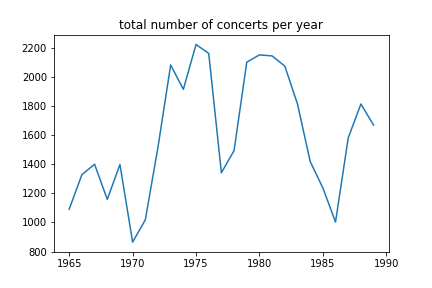
\includegraphics[width=83mm]{figures/TotalNumberofConcerts.png}
    \caption{Total number of concerts per year in the Michigan concert database from 1965 to 1990} \label {fig:num-concerts}
\end{figure}

Fig. \ref{fig:num-concerts} plots the total number of concerts per year in the concert database from the year 1965 to 1990. We observe that sharp changes in number of concerts occur around 1970 - 1975, and also around 1985. These changes are indeed reflected in the subsequent changepoint detection analysis. 
\begin{figure}[!ht]
 \centering
    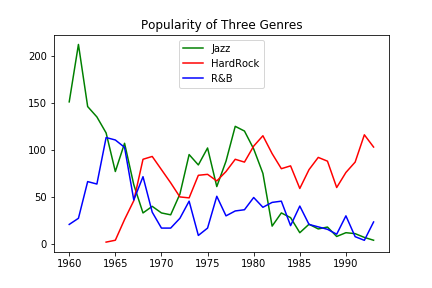
\includegraphics[width=83mm]{figures/ThreeGenres.png}
    \caption{Number of concerts per year for three top genres: Jazz, Hardrock, and RB} \label {fig:num-genres}
\end{figure}

Fig \ref{fig:num-genres} plots the number of concerts per year for the top three most ``popular" genres within the dataset. We see that the number of performances for each genre has non-trivial trends throughout the years 1960-1990. For example, Jazz as a genre has a resurgence around 1975, and HardRock is increasing in popularity after 1965. Note that since many of the concerts do not have genre information, the number of performances in this figure is an order of magnitude less than Fig. \ref{fig:num-concerts}. 


For the venue network, we define the edges by connecting venues that hosted a performance from the same artist during a predefined period of time. Namely, if the records (Artist, VenueA, t1) and  (Artist, VenueB, t2) are both found in the dataset with $t1 < t2 < t1 + T$, we place an undirected edge connecting VenueA to Venue B at time $t1$ rounded up to year. The parameter $T$ controls the connectivity of the graph. For this application, we choose $T = 1, 2, 3$. 

We observe consistent changes in the years xxx across all scales. We suspect these changes mainly reflect the fluctuations in number of concerts and the rise and fall of music genres since the changepoints correspond well visually to the fluctuations in Fig \ref{fig:num-concerts} and Fig \ref{fig:num-genres}.  The venue network seems to yield more interpretable results compared to the genre network. We suspect this is because genre information is too coarse for the network to accurately reflect true connections between subgroups of artists. 

\section{Temporal Motifs }
Temporal Motifs results.


\section{Graph Visualization }
Visualization of graph


\section{Future Work}

% Bibliography
\bibliography{pnsa}
\end{document}